\documentclass[parskip=half-]{scrreprt}
\parindent=0pt

\usepackage[ngerman]{babel}
\usepackage{amsmath}
\usepackage[T1]{fontenc}
\usepackage[utf8]{inputenc}
\usepackage{mathptmx}

\usepackage{graphicx}
\usepackage{amsmath}
\usepackage{caption}
\usepackage{xcolor}

\usepackage{geometry}
\geometry{a4paper, top=7mm, left=10mm, right=10mm, bottom=5mm, includefoot}


%enumnummerierung ebene2
\renewcommand{\labelenumii}{\arabic{enumii}}

%itemizeabstände
\usepackage{xpatch}
\xpatchcmd{\itemize}
  {\def\makelabel}
  {	\setlength{\itemsep}{0mm}
 	\setlength{\parskip}{0pt}
  	\setlength{\parsep}{0pt}  
  \def\makelabel}
  {}
  {}
  
  \xpatchcmd{\enumerate}
  {\def\makelabel}
  {	\setlength{\itemsep}{0mm}
 	\setlength{\parskip}{0pt}
  	\setlength{\parsep}{0pt}  
  \def\makelabel}
  {}
  {}

\renewcommand{\minisec}[1]{\textbf{#1}\\}
\newcommand{\Minisec}[1]{\textcolor{purple}{\minisec{#1}}}
\newcommand{\tabsec}[1]{\textcolor{purple}{\textbf{#1}}}


\newcommand{\includetablegraphics}[2]{
\begin{minipage}[t]{#1}
\includegraphics[width=\textwidth]{#2}
\end{minipage}
}



\newcommand{\dito}{$ \leadsto  $ ~}

\newcommand{\subtil}[1]{\textcolor{white!50!black!50}{#1}}

\begin{document}
	\begin{minipage}{0.45\textwidth}
%\Minisec{OSI-Modell}
\begin{tabular}{| p{0.3\textwidth} | p{0.15\textwidth} | p{0.55\textwidth} |}
\hline 
\textbf{ Schichtname}	& \textbf{Einheit} & \textbf{Regelt} \\
\hline 
Anwendungsschicht (Anwendungsschicht) & Nachrichten	& Funktionen für Anwendungen \\
\hline 
Darstellungsschicht  	& 		Nachrichten 	&Zeichensätze, Zahlendarstellung         \\
\hline 
Kommunikations- steuerungsschicht & Nachrichten	& Login\&Logout 			        \\
\hline 
Transportschicht	(Transportschicht)	&  Nachrichten	 & Übertragungsgarantie,
Reihenfolge, Fluss/Überlastkontrolle, Prozessadressierung, beliebige Nachrichtengröße  \\
\hline 
Vermittlungsschicht \mbox{(Internetschicht)}	&  Pakete 	& Routing						\\
\hline 
Sicherungsschicht   (Netzwerkschicht)	&  Frames	& Fehlererkennung/-korrektur, Medienzugriff, Framing, Zuverlässige Zustellung	\\
\hline 
Bitübertragungsschicht 	&  Bits 	& Frequenzen, Kabel, Kodierung  \\
\hline 
\end{tabular}
\end{minipage}\\
\rule{4cm}{0pt}
\begin{tabular}{|c|c|}
\hline
LLC - Link Logical Control 	& siehe Schicht 2 OSI		\\
\hline
MAC - Media Access Control 	& Medienzugriff)	\\
\hline
PHY - Physical Layer  		& Bitübertragung \\
\hline
\end{tabular}\\


	\Minisec{TCP/IP-Prüfsumme: }
\begin{minipage}{0.5\textwidth}
\begin{enumerate}
\item Aufsummieren aller 16-Bit-Blöcken in Einerkomplementdarstellung \\
\textbf{Einerrücklauf}(Wert / 65536)\\
Tatsächlicher Wert: mod 65536;\rule{2cm}{0pt} 65535 = 0; 
\item invertieren aller Prüfsummenbits (Erg = $65535 - $Wert)
\end{enumerate}
\end{minipage}
=> auf Empfängerseite muss $00 \dots 0 $ herauskommen\\
 

\newcommand{\Rx}[1]{\textcolor{blue}{#1}} 
\newcommand{\xx}[1]{\textcolor{cyan}{#1}}
\newcommand{\Ix}[1]{\textcolor{red}{#1}}
\newcommand{\Gx}[1]{\textcolor{brown}{#1}}
 
\Minisec{CRC (Cyclic Redundancy Check)}
\begin{minipage}{0.25\textwidth}
Bitkette $\Leftrightarrow$ Polynom, \\z.B. 1011 $\Leftrightarrow$ $x^3 + x ^1 + 1$\\
$+=-= $Xor\\\\
\Ix{I(x)} = Nutzdaten  \subtil{Informationspolynom}\\
\Gx{G(x)} = vorgegeben \subtil{Generatorpolynom }\\
\xx{k} = grad von G(x)\\
C(x) = Frame \subtil{Codepolynom}  \\\\
Berechnen: \Rx{R(x)} = \Ix{I(x)} $\cdot$ $\xx{x^k}$ mod \Gx{G(x)}; \rule{1cm}{0cm} \\
C(x) = \Ix{I(x)} $ \cdot \xx{x^k}$ +  \Rx{R(x)};\\
=> Empfänger prüft, ob C(x)/G(x) = 0;
\end{minipage}
\texttt{
\begin{minipage}{0.25\textwidth}
\newcommand{\divisor}{\underline{1011}\\}
\Ix{I= 100010,} \Gx{G(x)=$x^3 + x ^1 + 1 \widehat{=}1011$}\\
\textcolor{white}{|}\Ix{100010}\xx{000}:\Gx{1011}=101100\\
\textcolor{white}{|}\divisor
\textcolor{white}{|}001110\\
\textcolor{white}{|}~~\divisor
\textcolor{white}{|}~~01010\\
\textcolor{white}{|}~~~\divisor
\textcolor{white}{|}~~~000\textcolor{blue}{100 <= R(x)}\\
=> C(x) = \Ix{100010}\Rx{100}
\end{minipage}
}

	

\Minisec{Kodierungen}
\begin{tabular}{|c|c|c|c|}
\hline
	& \textbf{0} & \textbf{1} & \textbf{Beispiel} \\
\hline
NRZ	& 	0		& 	1	& \includetablegraphics{0.25\textwidth}{NRZ}				\\
\hline
NRZI & 	 halten	&	 ändern	&	\includetablegraphics{0.25\textwidth}{NRZI}			\\
\hline
Manchester &  $0 \rightarrow 1$ &  $1 \rightarrow 0$& 	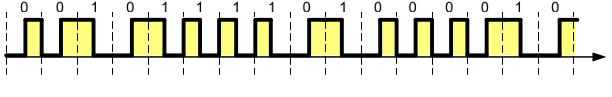
\includegraphics[width=0.25\textwidth]{Manchester}			\\
\hline
AMI 		& 0 & $\pm 1 $ & \ 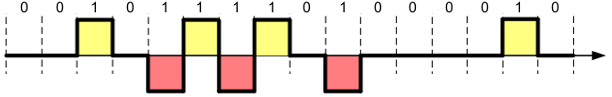
\includegraphics[width=0.25\textwidth]{AMI}	\\
\hline
\end{tabular}

\minisec{Code-Ersetzungen bei Ternären Codes (Rest wie bei AMI):}
\begin{tabular}{|c|c|c|}
\hline
Code:	& B8ZS &HDB3	\\
\hline
zu Ersetzen: & 8 Nullen	& 4	Nullen\\
\hline
Regel: 
&	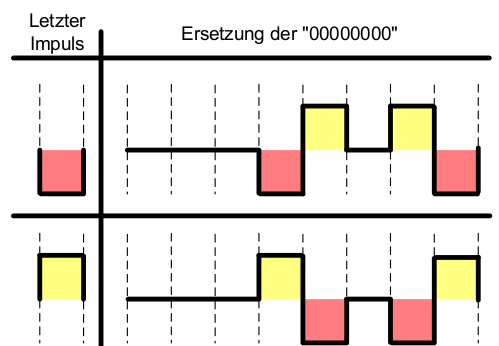
\includegraphics[width=0.2\textwidth]{B8ZS}		&	 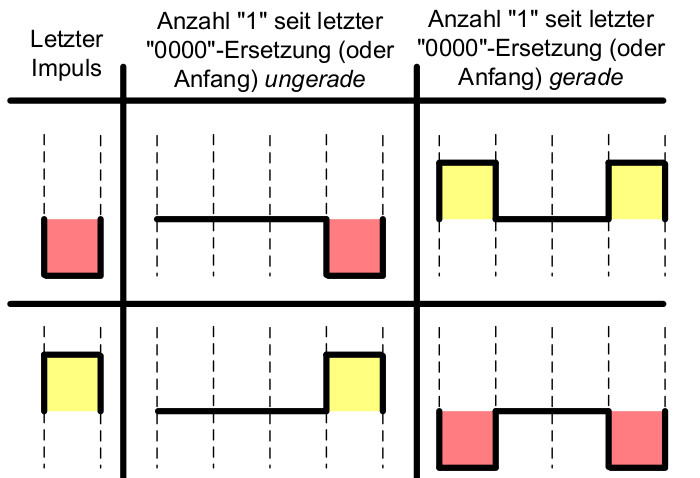
\includegraphics[width=0.2\textwidth]{HDB3} \\
\hline
\end{tabular}

\begin{minipage}{0.25\textwidth}
4B/5B mit maximal 3 Nullen in folge\\
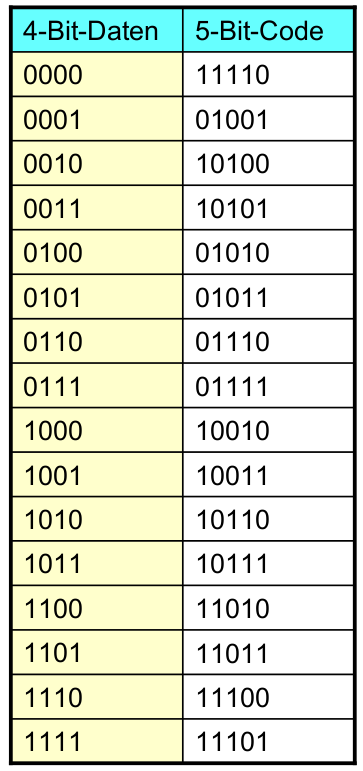
\includegraphics[angle=90 , width=\textwidth ]{4B5B}
\end{minipage}
\begin{minipage}{0.25\textwidth}
\centering
$ A = \log_2(B) \Leftrightarrow B = 2^A $
\end{minipage}

\newcommand{\formel}[1]{\fbox{$ #1 $}}
\newcommand{\tab}{\rule{0.5cm}{0pt}}

\Minisec{Übertragung}
\formel{v_{max} = 2 B;} \tab
\formel{D_{max} = 2 B \log_2(L)}\tab
\formel{D_{max} = B \log_2(1+ \frac{S}{N})}\tab
\formel{\frac{S}{N}= 10^{SNR[db]/10}}


$v_{max}$ = Schrittgeschwindigkeit; $D_{max}$ = Datenrate;	 B = Bandbreite; \\
L = Signalstufen; 	SNR = Signal-Rausch-Abstand [db]







\clearpage	
	
	\Minisec{Link-State-Routing}
\Minisec{Dijkstra}
\begin{minipage}[t]{0.25\textwidth}
Menge M:=schon abgearbeitete Knoten; \\
Baum B:= gesuchter Quellbaum \\
di:= berechneter Abstand zu Ni \\
 
\textbf{initialisiere: }\\
Startknoten in M und B einfügen, \\
di=Wert der Kante Ni zu Startknoten, sonst $\infty$

\textbf{Bis alle Knoten in M sind: }
\begin{enumerate}
\item \textcolor{red}{suche das kleinste di, }
\item füge diesen Knoten Ni zu M hinzu, 
\item füge die kürzeste Kante von B zu Ni in B ein.
\item passe die d der Nachbarn von Ni an, wenn di + Kante von Ni kürzer ist
\end{enumerate}

\end{minipage}
\begin{minipage}[t]{0.25\textwidth}
Bsp: Startknoten: $N_1$\\
\begin{tabular}{|l|l|c|c|c|}
\hline
Runde 	&	M 			& $d_2$		& $d_3$			& $d_4$\\	\hline
1	&	{$N_1$} 	& \textcolor{red}{1}	& 3 &	 $\infty$ \\ \hline
2	&	{$N_1$, $N_2$} 	&  		& 	\textcolor{red}{2}	 & 3 \\ \hline
3	&	{$N_1$, $N_2$, $N_3$} 	& 		& 	 & \textcolor{red}{3} \\ \hline
\end{tabular}\\
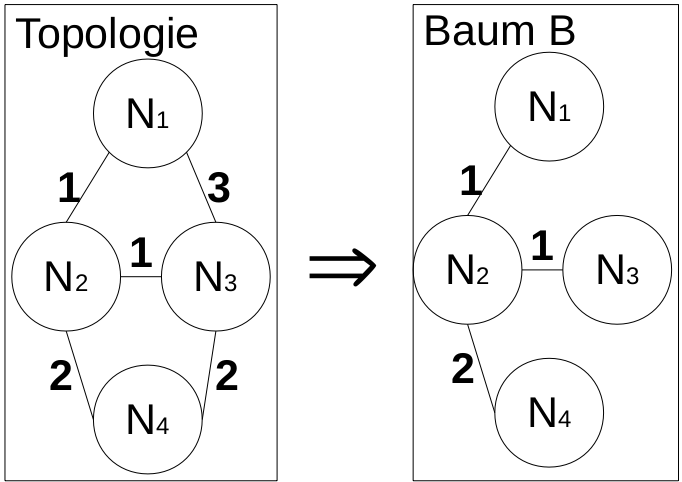
\includegraphics[width=\textwidth]{Dijkstra}
\end{minipage}\\\\

\begin{minipage}{0.25\textwidth}
\Minisec{OLSR - MPR}
Fluten nur an ausgewählte Nachbarn.\\
N(K):= Nachbarn von K \\
N2(K):= Nachbarsnachbarn von K \\
MPR(K):= Weiterflutende knoten in N(K)
\end{minipage} 			
\begin{minipage}{0.25\textwidth}
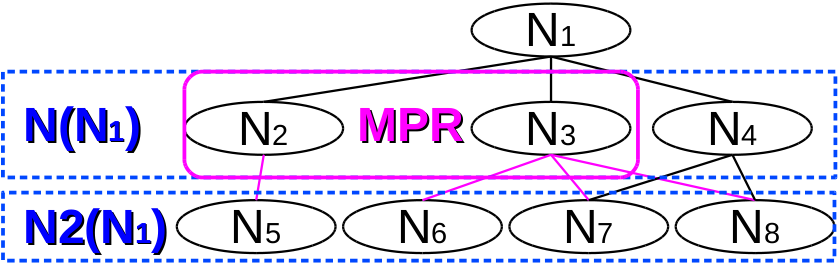
\includegraphics[width=\textwidth]{OLSR}
\end{minipage} 

\begin{enumerate}
\item MPR = Knoten in N(K), die einzige Verbindung eines Knotens in N2(K) sind (Bsp: $N_2$)
\item Solange noch nicht alle Knoten in N2 erreicht werden:\\
Suche den Knoten aus N(K), der die meisten fehlenden Knoten in N2(K) erreicht und füge ihn zu MPR hinzu ($N_3$) \\
(bei mehreren Kandidaten denjenigen mit meisten Nachbarn)
\item Entferne Knoten, wenn danach immer noch alle Knoten in N2(K) erreicht werden
\end{enumerate}

\Minisec{Link-Reversal-Routing}
Weg zu einem Ziel: Directed Acyclic Graph (DAG)\\
\begin{minipage}{0.5\textwidth}
\begin{enumerate}
\item Full Reversal: hat ein Knoten nur eingehende Kanten: drehe alle um
\item Partial Reversal (listenbasiert): Knoten führen Liste über von Nachbarn gedrehte Kanten; sind alle Kanten drin lösche die Liste\\
gibt es nur eingehende Kanten drehe alle Kanten um, die nicht in der Liste stehen; 
\end{enumerate}
\end{minipage}




\Minisec{DBF:}
Jeder Knoten hat eine Tabelle mit Ziel, Hop zum Ziel, Metrik(Kosten);\\
\begin{minipage}{0.5\textwidth}
\begin{tabbing}
\textbf{Initialisierung:} \= Loopback mit Metrik 0 eintragen;\\
\> Verbindung zu den Nachbarn mit der gemessenen Metrik eintragen\\
\> Alle Anderen Verbindungen: Hop = ? Metrik= $\infty$
\end{tabbing}
\end{minipage}

\textbf{Abgleich mit Nachbartabelle:} In jeder Zeile prüfen: \\
\begin{minipage}{0.5\textwidth}
\begin{itemize}
\item Berechne Eintrag der Nachbartabelle + Verbindungsmetrik
\item Ist der Nachbar der Hop der Zeile: Übernimm veränderten Wert
\item Ist die Route über den Nachbarn besser $\rightarrow$ Nachbarn als Hop mit Metrik eintragen
\end{itemize}
\end{minipage}

\textbf{Count-To-Infinity-Problem:} nach Verbindungsabbruch evtl. Feedback-Schleife  \\
\begin{minipage}{0.5\textwidth}
\begin{itemize}
\item definiere kleinen Wert als Unendlich
\item Split Horizon: Zeilen werden nicht dem eingetragenen Hop weitergereicht 
\item Versionsnummern der Einträge (DSDV)
\end{itemize}
\end{minipage}\\

\Minisec{DSDV:}
DBF Tabelle um Spalte für Sequenznummer erweitern (mit -1 initialisiert)

\textbf{Abgleich mit Nachbartabelle:} \underline{höhere} Sequenznummer gewinnt (\underline{Gleiche:} siehe DBF)

\textbf{Nach Abgleich mit allen Nachbarn} :  \textit{Eigene} Sequenznummer +2 ~~(Metrik=0);\\
\textbf{ Verbindungsabbruch} zu Nachbarn Nx: in alle Zeilen mit Hop = Nx: \\
\rule{1cm}{0pt} Metrik = $\infty$ Hop = ? Sequenznummer++





\Minisec{IPv6}
Adressen: 8 4er-Blöcke(Hex) z.B. 47cd::22:1234:a456:12 \\
64 Bit Präfix(Netzwerkanteil) 64 Bit Interface Identifier\\
\begin{tabular}{|c|c|}
\hline
Adressen & Funktion \\ \hline
::1 		& Local Loopback \\ \hline
fe80::/10 	& Link Local Unicast (Autokonfiguration) \\ \hline
fc00::/7	& Unique Local Unicast (Private Adressen) \\ \hline
ff00::/8	& Multicast (Broadcast mit verschiedenen Reichweiten) \\ \hline
weitere:	& Anycast (Route an irgendeinen Host einer speziellen Gruppe) \\ \hline
\end{tabular}\\

\textbf{Autoconfiguration: }\\
\begin{minipage}{0.5\textwidth}
\begin{enumerate}
\item Berechne Identifier (aus MAC oder zufällig)
\item => frage bei Router mit fe801::/64 + Identifyer (Link Local Unicast Adresse)
\item Router teilt mögliche Präfixe mit
\item Host prüft ob Adresse schon vorhanden (Double Address Detection)
\end{enumerate}
\end{minipage}\\


\textbf{DHCP: }\\
\begin{minipage}{0.5\textwidth}
\begin{enumerate}
\item Client: DHCPDISCOVER (per Broadcast)
\item Server: DHCPOFFER 
\item Client: DHCPREQUEST
\item Server: DHCPACK (Client hat nun Adresse geleast)
\end{enumerate}
\end{minipage}
\clearpage




\tabsec{IPv4} Hostanteil $1\dots1$= Broadcast  $0\dots0$= Netzadresse \\
\begin{tabular}{|c|c|c|c|}	
\hline
Klasse & Von & bis &  \\
\hline
A 	& 0.0.0.0 	& 127.255.255.255 & 16.777.214 Hosts	\\
\hline
B	& 128.0.0.0 & 191.255.255.255 & 65.534 Hosts		\\
\hline
C	& 192.0.0.0 & 223.255.255.255 & 254	Hosts	\\
\hline
D	& 224.0.0.0 & 239.255.255.255 & Multicast 	\\
\hline
E	& 240.0.0.0	& 255.255.255.255 & Reserviert 	\\
\hline	
 & 127.0.0.0 & 127.255.255.255 & Loopback 	\\
 \hline
A & 10.0.0.0 & 10.255.255.255 & privat 	\\
 \hline
B & 172.16.0.1 & 172.31.255.255& privat  	\\
 \hline
C & 192.168.0.1 & 192.168.255.255 & privat  	\\
 \hline
\end{tabular}~~~~
\begin{tabular}{|c|c|}
\hline
Oktett & Bits \\ \hline
255 & 1111 1111 \\ \hline
254 & 1111 1110 \\ \hline
252 & 1111 1100 \\ \hline
248 & 1111 1000 \\ \hline
240 & 1111 0000 \\ \hline
224 & 1110 0000 \\ \hline
192 & 1100 0000 \\ \hline
128 & 1000 0000 \\ \hline
\end{tabular}

\minisec{Fragmentieren}
Ident(16Bit) ID eines \underline{Pakets}, Offset(13Bit): Position des Fragments \textbf{\textcolor{red}{/ 8}}	\\
Fragmentierungsbit: 1=verboten, More: 1=weitere , 0=letztes Fragment	

\minisec{Vorgehen}
Größtmögliche Pakete herausschneiden, evtl ein kleinerer Rest im letzten Paket.\\
\textbf{Beachten:} Fragmentieren auf \textcolor{red}{Vielfache von 8} z.B. 512,520... u.U. IP-Header 20Byte \\
Router "defragmentieren" \textbf{nicht}; 


%\clearpage	
	
	\Minisec{TCP}
Nagle: Sende wenn MTU erreicht oder alle bisher gesendeten Segmente bestätigt

\newcommand{\ack}{\textcolor{green!50!black!90!}{\textbf{Acknowledge}}}
\newcommand{\advert}{\textcolor{blue}{\textbf{Advertised Window}}}

\minisec{Sliding Window}
Empfänger antwortet mit: ( \ack ,\advert) \\
\ack: nextByteExpected -1  \\
\advert = maxRecieveBuffer - (lastByteRecieved - lastByteRead)

Sender kann Senden:\\
Effective Window = \advert - (LastByteSent - LastByteAcked)\\
Bei Effective Window = 0: Sender sendet periodisch 1 Byte (bis Effective Window steigt)

\minisec{Timeouts}
$RTT_{Last}$: gemessener RTT\\
$RTT = a \cdot RTT + (1-a) \cdot RTT_{Last}$\\
\begin{minipage}{0.5\textwidth}
\begin{itemize}
\item Timeout = 2* RTT
\item Deviation = Deviation $\cdot$ a + $|RTT_{Last} -RTT| \cdot (1-a)$\\
Timeout = RTT + 4$\cdot$Deviation
\end{itemize}
\end{minipage}

\minisec{Überlastkontrolle}
\minisec{Additive-Increase/Multiplicative-Decrease:}
beginne mit Congestionwindow = 1; bei ACK ++ ; bei Timeout /2;   \\
\minisec{Slow Start: }
bei Start, nachdem Datenrate auf 0 gefallen: erhöhe CongestionWindow durch *2






\Minisec{DNS}
Namensraum:bis 255 Zeichen aus verketteten Labels; \\
Labels: 1-63 Zeichen aus a-z,0-9 und -; Sonderzeichen mit Punycode\\
Records: Zuordnugstabellen Typen: A (IPv4) AAAA (IPv6) PTR (Reverse Lookup) ...

\minisec{organisatorische Struktur:} aufteilung in Zonen (Domain und darunterliegende Hosts); \\
jede Zone hat eigene Nameserver, Verantworlichen und Namenskonventionen\\
Nameserver kennen: direkt untergeordnete Hosts und Nameserver;  Root-Server


\minisec{Auflösungsmechanismus:}
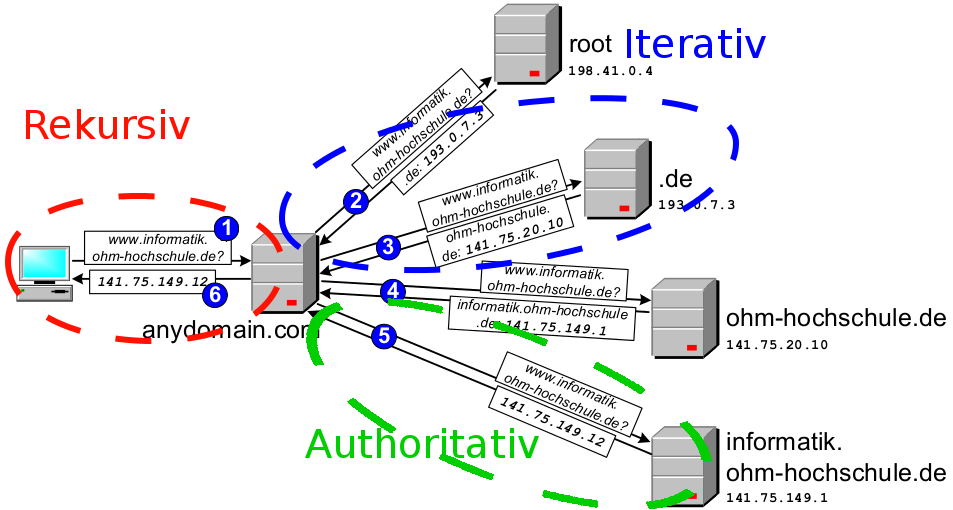
\includegraphics[width=0.3\textwidth]{DNS}

\minisec{Reverse-Lookup:}
Umwandeln der IP-Adresse in spezielle Domain, anfrage in Record PTR\\
TLDs: in-addr.arpa, ip6.arpa\\
z.B. 141.75.201.12 $\rightarrow$ 12.201.75.141.in-addr.arpa 

\Minisec{DNSsec}
Antwort wird signiert, Schlüssel durch nächsthöheren DNS bestätigt \\
2 Schlüsselpaare (Erleichtert Schlüsseltausch, kurze Schlüssel möglich):\\
\textbf{ZSK} (Zone Signing Key): Signieren der Antworten (kurz, Änderung Tage-Wochen), Tausch hat nur lokale Auswirkungen\\
\textbf{KSK} (Key Signing Key): Signieren der Schlüssel (lang, Änderung Jahre), Bei Tausch absprache mit übergeordneten Domain

\textcolor{red}{\textbf{DS}} (Delegation Signer): Mit ZSK signierter öffentlicher KSK der \textbf{Subdomain}

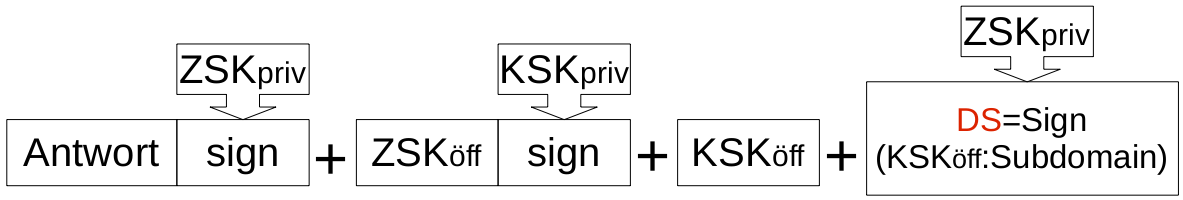
\includegraphics[width=0.4\textwidth]{DNSsec}

\Minisec{URL}
Protokoll :// Benutzer : Passwort @ Domain : Port / Pfad ? Anfrage \# Abschnitt	
	

\clearpage	
	
%	% --- Schicht 7
\Minisec{Anwendungskommunikation}
Request-Response-Paradigma: Anfrage->Antwort\\
Textbasierte-Protokolle: (z.B. smtp,http), Vorteile: debuggen, leicht zu Dokumentieren(RFC)

\Minisec{http}
Form: Kommandozeile, Headerzeilen, Leerzeile, [Bodyzeilen] (Bodyende: Headerfeld oder End-Tags)\\
Kommandozeile: Methode(GET,$\dots$) Anfrage-URI Version

Persistente Verbindung: Nutzen einer TCP-Verbindung für mehrere HTTP-REQUESTS (Flusskontrolle, Handshake)\\
Pipelining: Client stellt mehrere Anfragen über eine Verbindung bevor erste Antwort kommt\\
Long Polling: Server antwortet nicht sofort, sondern nur bei Ereignis oder Timeout (asynchronität)\\
zustandslos => keine Sitzungen (Benutzeridentifikation) => SitzungsID in Cookie oder URL

\Minisec{Web-Sockets}
Bidirektionale Kommunikation über einen durch http etablierten Kanal => Zuordnung zu Sitzung leicht möglich\\
Nach dem Aufbau verwendung eigenes Format (kein Http): Längenangabe einzelner Nachrichten, zufallsmaskierung gegen Proxie-Caching

\Minisec{Remote Procedure Call}
Aufruf von Funktionen/Methoden auf entferntem Rechner z.B. RPC, CORBA(Sprachenunabhängig), RMI(Java)\\
Nötig: Stubs auf Client/Server, die die Kommunikation übernehmen, plattformunabhängige Kodierung der Daten und Serialisierung(abrollen von Objekten) 

\Minisec{Webservices}
HTTP als Quasi-Transportprotokoll (wird nicht blockiert,...) \\
v.A. für Kommunikation zwischen verschiedenen Verantwortungsbereichen z.B. Amazon $\longleftrightarrow$ DHL

\minisec{SOAP}
Definition von Operationen (mit Parametern, Rückgabe ...)\\
Schnittstellenbeschreibung in WSDL, wird über HTTP übertragen => Prüfen auf Aktuelle Version, Stubgenerierung möglich

\minisec{REST}
Zugriff auf Ressourcen über HTTP-Kommandos mit URIs, Argumente im Body, Rückgabe in Content-Feld\\
z.B. GET http://abookstore/cart/12345\\
Format z.B. in JSON / XML; Kommandos GET, PUT, POST, DELETE



	\Minisec{Chord}
Fingertabelle für einen Host A:\\
\begin{tabular}{c|c|c|c}
k & start & end & Node \\
\hline
1	& 	$A_{end}+1$ & nächster Start-1 & Host mit start in Hashtable	\\
2 	&  \dito +1 		&  "				& suche start in Hashtable 	\\
3 	&  \dito +2 		& "					& \\
4  &  \dito +4 			&   "				& \\
k  &  $\cdots$		&  $A_{end}-1$	 	& \\
\end{tabular} \\

\begin{minipage}{0.2\textwidth}
z.B. Fingertabelle für A mit DHT
(Hashlänge = 5 => rechnen mod 32) 

\begin{tabular}{|c|c|c|}
\hline
Knoten & Start & Ende \\
\hline
B & 5 & 14\\
\hline
A & 15 & 20 \\
\hline
C & 21 & 4 \\
\hline
\end{tabular}
\end{minipage} \textbf{$\implies$}
\begin{minipage}{0.25\textwidth}
\begin{tabular}{c|c|c|c}
k & start & end & Node\\
\hline
1	& 	21 & 21 & C\\
2 	&   22 		&  23	&		C		\\
3 	&   24		& 27	&	C \\
4  &  	28		&   3	& C	\\
5 & 4			&	19 &  B
\end{tabular}
\end{minipage}\\

\textbf{Join:} Vorraussetzung: Bekannter Rechner n';

\begin{minipage}{0.5\textwidth}
\begin{enumerate}
\item zuständigkeitsbereich ausrechnen (Hashen der Adresse) und zuständigen Host suchen
\item Fingertabelle anlegen (lookup durch n')
\item Anpassen aller Fingertabellen, die auf den neuen Rechner zeigen \\
(ist abhängig von der größe des übernommenen Hashbereichs)
\item Übernehmen der relevanten Einträge vom bisher zuständigen Host
\end{enumerate}
\end{minipage}\\

\Minisec{CAN}
Abbilden der Hashes auf d Dimensionen\\
Knoten verwaltet Hashes in einem d-Dimensionalen Quader und seine direkten Nachbarn.\\
\textbf{Suche:} Anfrage an den dem Ziel nähesten Nachbarn (Distanz vom Mittelpunkt)\\
\textbf{Join:} wähle zufälligen Punkt, halbiere Bereich (wenn möglich zu Quadraten)	\\
\textbf{Leave:} Übergabe des Quaders an einen Nachbarn \\
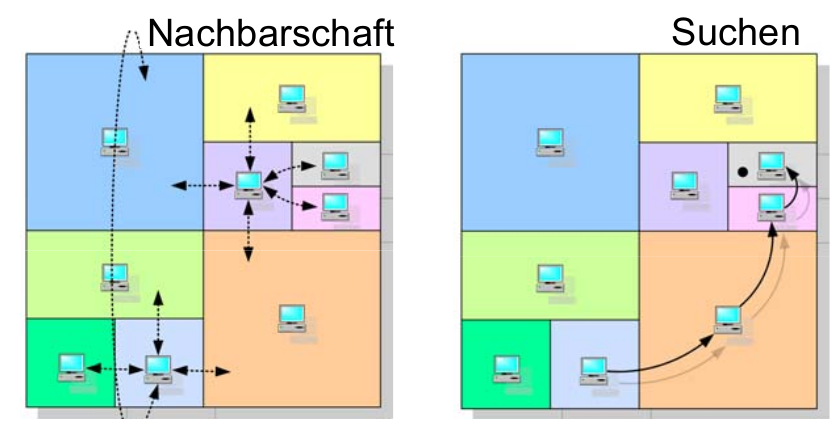
\includegraphics[width=0.35\textwidth]{CAN}


	
	\Minisec{Sicherheit}
Sicherheitsziele: Vertraulichkeit, Authentizität, Integrität, Anonymität, $\dots$


\Minisec{Betriebsmodi: }
Codebook Mode: Jeder Block einzeln verschlüsselt\\
CBC: Änderung der Nachricht => keine Mustererkennung\\
Counter mode: Simuliert Stromchiffre mit Pseudozufallsgenerator (aus Nonce)\\
\begin{tabular}{cc}
\textbf{Cypher Block Chaining} & \textbf{Counter Mode}\\
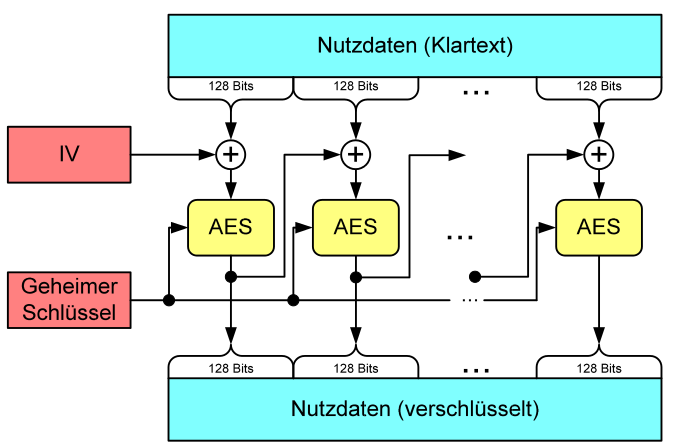
\includegraphics[width=0.25\textwidth]{CBC}   &  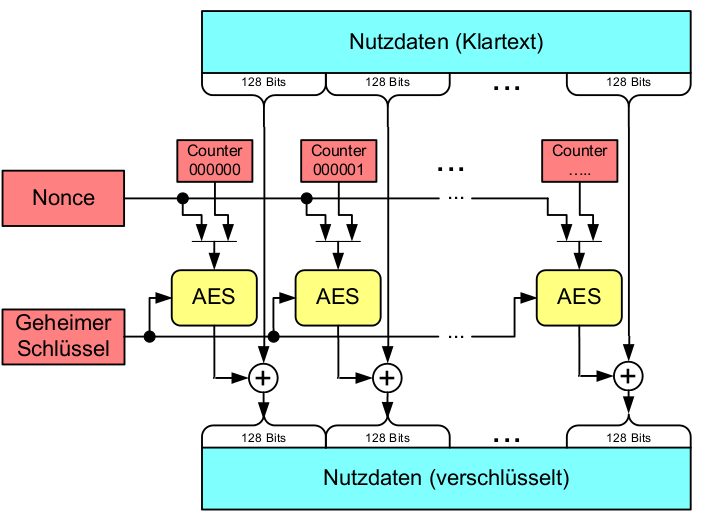
\includegraphics[width=0.25\textwidth]{Counter}\\
\end{tabular}




\Minisec{Rainbow Table: }
\textbf{Erstellen einer Zeile:} beginne bei Startwert, wiederhole Hash- und Reduktionsfunktion bis zum k-ten Hashwert (k=Kettenlänge), speichere Start und Endwert (letzter Hash);\\
\textbf{suchen:} wiederhole Hash und Reduktion bis ein bekannter Endwert, dann gehe vom Startwert mit Hash und Reduktion bis gesuchter Wert erreicht wird\\
\textbf{Salzen:} erzeugen und Speichern von Zufallszahl, hashen von Passwort und Salz

	% --- Schicht 7



\Minisec{http}
\textbf{Persistente Verbindung:} eine TCP-Verbindung für mehrere HTTP-REQUESTS\\
\textbf{Pipelining:} Client stellt mehrere Anfragen ohne warten auf Antwort \\
\textbf{Long Polling:} Server antwortet erst nach Ereignis oder Timeout (asynchronität)\\
\textbf{zustandslos} => keine Sitzungen => SitzungsID in Cookie oder URL


\Minisec{Webservices}
\minisec{SOAP}
Definition von Operationen (mit Parametern, Rückgabe ...)\\
Schnittstellenbeschreibung mit WSDL => Prüfen auf Aktuelle Version, Stuberzeugung möglich

\minisec{REST}
Zugriff auf Ressourcen über HTTP-Kommandos mit URIs\\
z.B. GET http://abookstore/cart/12345


	
\end{document}